\documentclass{standalone}
\usepackage{tikz}
\usetikzlibrary{patterns}
\usetikzlibrary{positioning}
\usetikzlibrary{patterns, positioning}
\usetikzlibrary{shapes.misc}
\usepackage[outline]{contour}
\contourlength{1.5pt} 
\usetikzlibrary{calc}
        \usepackage{relsize}
        \tikzset{fontscale/.style = {font=\relsize{#1}}}

\begin{document}
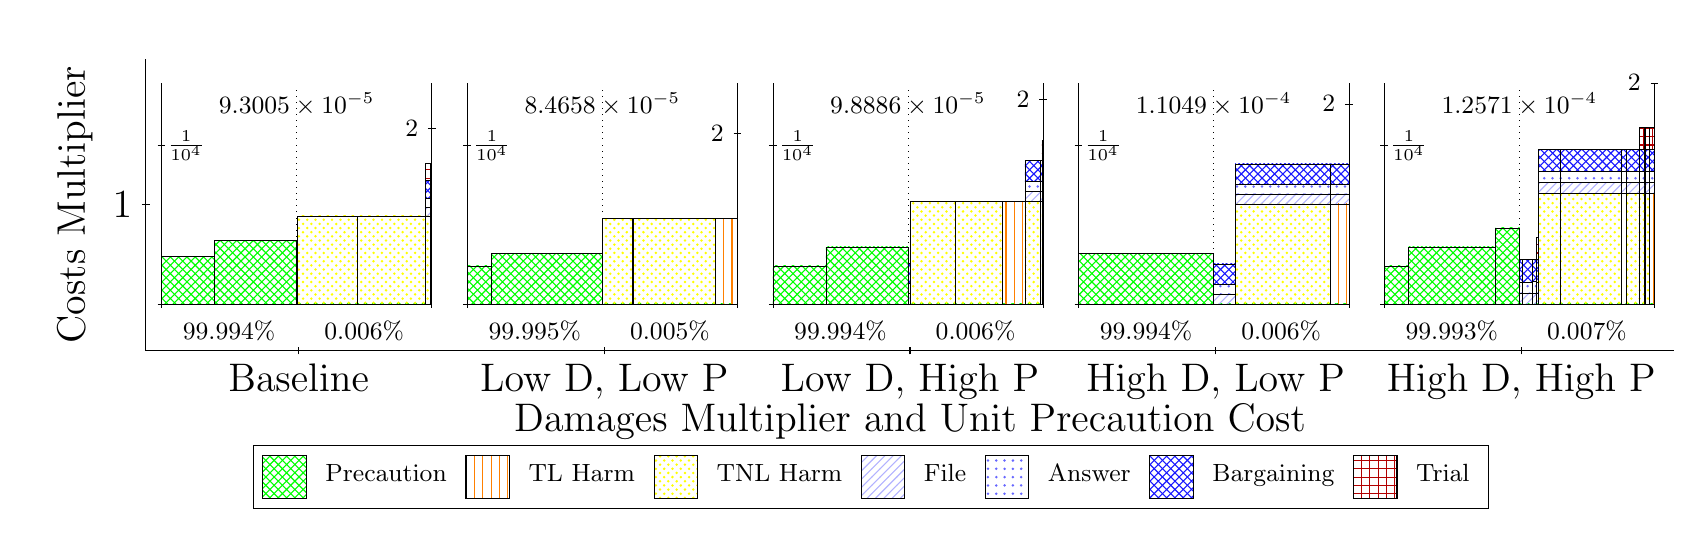
\begin{tikzpicture}
\clip(-0.5,-1.1) rectangle +(20.91,6.2);
\draw[black] (1,1) -- (1,4.7);
\node[rotate=90, fontscale=2, anchor=center] at (0.1, 2.85) {Costs Multiplier};
\draw[black] (0.95,2.85) -- (1.05,2.85);
\node[fontscale=2, anchor=east] at (0.95, 2.85) {1};

\draw[black] (1,1) -- (20.41,1);
\node[fontscale=2, anchor=center] at (10.705, 0.1) {Damages Multiplier and Unit Precaution Cost};
\draw[black] (2.941,0.95) -- (2.941,1.05);
\node[fontscale=2, anchor=north] at (2.941, 0.95) {Baseline};
\draw[black] (6.823,0.95) -- (6.823,1.05);
\node[fontscale=2, anchor=north] at (6.823, 0.95) {Low D, Low P};
\draw[black] (10.705,0.95) -- (10.705,1.05);
\node[fontscale=2, anchor=north] at (10.705, 0.95) {Low D, High P};
\draw[black] (14.587,0.95) -- (14.587,1.05);
\node[fontscale=2, anchor=north] at (14.587, 0.95) {High D, Low P};
\draw[black] (18.469,0.95) -- (18.469,1.05);
\node[fontscale=2, anchor=north] at (18.469, 0.95) {High D, High P};


\draw[pattern=crosshatch, pattern color=green,draw=black,very thin] (1.2,1.592) rectangle (1.8725,2.1945);
\draw[pattern=crosshatch, pattern color=green,draw=black,very thin] (1.8725,1.592) rectangle (2.916,2.3954);
\draw[pattern=crosshatch, pattern color=green,draw=black,very thin] (2.916,1.592) rectangle (2.9287,1.592);
\draw[pattern=north east lines, pattern color=blue!30,draw=black,very thin] (2.916,1.592) rectangle (2.9287,1.7037);
\draw[pattern=dots,  pattern color=blue!60,draw=black,very thin] (2.916,1.7037) rectangle (2.9287,1.8154);
\draw[pattern=crosshatch,      pattern color=blue!90,draw=black,very thin] (2.916,1.8154) rectangle (2.9287,2.0388);
\draw[pattern=grid,            pattern color=red!70!black,draw=black,very thin] (2.916,2.0388) rectangle (2.9287,2.2621);
\draw[pattern=crosshatch, pattern color=green,draw=black,very thin] (2.9287,1.592) rectangle (3.6818,1.592);
\draw[pattern=crosshatch dots, pattern color=yellow,draw=black,very thin] (2.9287,1.592) rectangle (3.6818,2.7089);
\draw[pattern=crosshatch, pattern color=green,draw=black,very thin] (3.6818,1.592) rectangle (3.6897,1.592);
\draw[pattern=vertical lines, pattern color=orange,draw=black,very thin] (3.6818,1.592) rectangle (3.6897,2.7089);
\draw[pattern=crosshatch, pattern color=green,draw=black,very thin] (3.6897,1.592) rectangle (4.5556,1.592);
\draw[pattern=crosshatch dots, pattern color=yellow,draw=black,very thin] (3.6897,1.592) rectangle (4.5556,2.7089);
\draw[pattern=crosshatch, pattern color=green,draw=black,very thin] (4.5556,1.592) rectangle (4.6122,1.592);
\draw[pattern=crosshatch dots, pattern color=yellow,draw=black,very thin] (4.5556,1.592) rectangle (4.6122,2.7089);
\draw[pattern=north east lines, pattern color=blue!30,draw=black,very thin] (4.5556,2.7089) rectangle (4.6122,2.8205);
\draw[pattern=dots,  pattern color=blue!60,draw=black,very thin] (4.5556,2.8205) rectangle (4.6122,2.9322);
\draw[pattern=crosshatch,      pattern color=blue!90,draw=black,very thin] (4.5556,2.9322) rectangle (4.6122,3.1556);
\draw[pattern=grid,            pattern color=red!70!black,draw=black,very thin] (4.5556,3.1556) rectangle (4.6122,3.379);
\draw[pattern=crosshatch, pattern color=green,draw=black,very thin] (4.6122,1.592) rectangle (4.632,1.592);
\draw[pattern=vertical lines, pattern color=orange,draw=black,very thin] (4.6122,1.592) rectangle (4.632,2.7089);
\draw[pattern=north east lines, pattern color=blue!30,draw=black,very thin] (4.6122,2.7089) rectangle (4.632,2.8205);
\draw[pattern=dots,  pattern color=blue!60,draw=black,very thin] (4.6122,2.8205) rectangle (4.632,2.9322);
\draw[pattern=crosshatch,      pattern color=blue!90,draw=black,very thin] (4.6122,2.9322) rectangle (4.632,3.1556);
\draw[pattern=grid,            pattern color=red!70!black,draw=black,very thin] (4.6122,3.1556) rectangle (4.632,3.379);
\node[font=\small,text=black,anchor=north] at (2.916, 4.4) {$9.3005\times 10^{-5}$};
\draw[black,very thin] (1.2,1.592) -- (1.2,4.4);
\draw[black,very thin] (1.15,1.592) -- (1.25,1.592);
\node[font=\small,text=black, anchor=west] at (1.15, 1.592) {};
\draw[black,very thin] (1.15,3.6004) -- (1.25,3.6004);
\node[font=\small,text=black, anchor=west] at (1.15, 3.6004) {$\frac{1}{10^{4}}$};

\draw[black,dotted,very thin] (2.916,1.6762) -- (2.916,4.3158);
\draw[black,very thin] (4.632,1.592) -- (4.632,4.4);
\draw[black,very thin] (4.582,3.8257) -- (4.682,3.8257);
\node[font=\small,text=black, anchor=east] at (4.582, 3.8257) {\contour{white}{2}};

\draw[black,very thin] (1.2,1.592) -- (4.632,1.592);
\draw[black,very thin] (1.2,1.542) -- (1.2,1.642);
\node[font=\small,text=black, anchor=north] at (1.2, 1.542) {};
\draw[black,very thin] (4.632,1.542) -- (4.632,1.642);
\node[font=\small,text=black, anchor=north] at (4.632, 1.542) {};

\node[font=\small,text=black,anchor=south] at (2.058, 0.992) {99.994\%};
\node[font=\small,text=black,anchor=south] at (3.774, 0.992) {0.006\%};

\draw[pattern=crosshatch, pattern color=green,draw=black,very thin] (5.082,1.592) rectangle (5.3844,2.074);
\draw[pattern=crosshatch, pattern color=green,draw=black,very thin] (5.3844,1.592) rectangle (6.798,2.2347);
\draw[pattern=crosshatch, pattern color=green,draw=black,very thin] (6.798,1.592) rectangle (6.7985,1.592);
\draw[pattern=north east lines, pattern color=blue!30,draw=black,very thin] (6.798,1.592) rectangle (6.7985,1.7005);
\draw[pattern=dots,  pattern color=blue!60,draw=black,very thin] (6.798,1.7005) rectangle (6.7985,1.809);
\draw[pattern=crosshatch,      pattern color=blue!90,draw=black,very thin] (6.798,1.809) rectangle (6.7985,2.026);
\draw[pattern=grid,            pattern color=red!70!black,draw=black,very thin] (6.798,2.026) rectangle (6.7985,2.243);
\draw[pattern=crosshatch, pattern color=green,draw=black,very thin] (6.7985,1.592) rectangle (7.1737,1.592);
\draw[pattern=crosshatch dots, pattern color=yellow,draw=black,very thin] (6.7985,1.592) rectangle (7.1737,2.677);
\draw[pattern=crosshatch, pattern color=green,draw=black,very thin] (7.1737,1.592) rectangle (7.1968,1.592);
\draw[pattern=vertical lines, pattern color=orange,draw=black,very thin] (7.1737,1.592) rectangle (7.1968,2.677);
\draw[pattern=crosshatch, pattern color=green,draw=black,very thin] (7.1968,1.592) rectangle (8.2367,1.592);
\draw[pattern=crosshatch dots, pattern color=yellow,draw=black,very thin] (7.1968,1.592) rectangle (8.2367,2.677);
\draw[pattern=crosshatch, pattern color=green,draw=black,very thin] (8.2367,1.592) rectangle (8.5111,1.592);
\draw[pattern=vertical lines, pattern color=orange,draw=black,very thin] (8.2367,1.592) rectangle (8.5111,2.677);
\draw[pattern=crosshatch, pattern color=green,draw=black,very thin] (8.5111,1.592) rectangle (8.5118,1.592);
\draw[pattern=crosshatch dots, pattern color=yellow,draw=black,very thin] (8.5111,1.592) rectangle (8.5118,2.677);
\draw[pattern=north east lines, pattern color=blue!30,draw=black,very thin] (8.5111,2.677) rectangle (8.5118,2.7855);
\draw[pattern=dots,  pattern color=blue!60,draw=black,very thin] (8.5111,2.7855) rectangle (8.5118,2.894);
\draw[pattern=crosshatch,      pattern color=blue!90,draw=black,very thin] (8.5111,2.894) rectangle (8.5118,3.111);
\draw[pattern=grid,            pattern color=red!70!black,draw=black,very thin] (8.5111,3.111) rectangle (8.5118,3.328);
\draw[pattern=crosshatch, pattern color=green,draw=black,very thin] (8.5118,1.592) rectangle (8.514,1.592);
\draw[pattern=vertical lines, pattern color=orange,draw=black,very thin] (8.5118,1.592) rectangle (8.514,2.677);
\draw[pattern=north east lines, pattern color=blue!30,draw=black,very thin] (8.5118,2.677) rectangle (8.514,2.7855);
\draw[pattern=dots,  pattern color=blue!60,draw=black,very thin] (8.5118,2.7855) rectangle (8.514,2.894);
\draw[pattern=crosshatch,      pattern color=blue!90,draw=black,very thin] (8.5118,2.894) rectangle (8.514,3.111);
\draw[pattern=grid,            pattern color=red!70!black,draw=black,very thin] (8.5118,3.111) rectangle (8.514,3.328);
\node[font=\small,text=black,anchor=north] at (6.798, 4.4) {$8.4658\times 10^{-5}$};
\draw[black,very thin] (5.082,1.592) -- (5.082,4.4);
\draw[black,very thin] (5.032,1.592) -- (5.132,1.592);
\node[font=\small,text=black, anchor=west] at (5.032, 1.592) {};
\draw[black,very thin] (5.032,3.6004) -- (5.132,3.6004);
\node[font=\small,text=black, anchor=west] at (5.032, 3.6004) {$\frac{1}{10^{4}}$};

\draw[black,dotted,very thin] (6.798,1.6762) -- (6.798,4.3158);
\draw[black,very thin] (8.514,1.592) -- (8.514,4.4);
\draw[black,very thin] (8.464,3.762) -- (8.564,3.762);
\node[font=\small,text=black, anchor=east] at (8.464, 3.762) {\contour{white}{2}};

\draw[black,very thin] (5.082,1.592) -- (8.514,1.592);
\draw[black,very thin] (5.082,1.542) -- (5.082,1.642);
\node[font=\small,text=black, anchor=north] at (5.082, 1.542) {};
\draw[black,very thin] (8.514,1.542) -- (8.514,1.642);
\node[font=\small,text=black, anchor=north] at (8.514, 1.542) {};

\node[font=\small,text=black,anchor=south] at (5.94, 0.992) {99.995\%};
\node[font=\small,text=black,anchor=south] at (7.656, 0.992) {0.005\%};

\draw[pattern=crosshatch, pattern color=green,draw=black,very thin] (8.964,1.592) rectangle (9.6365,2.074);
\draw[pattern=crosshatch, pattern color=green,draw=black,very thin] (9.6365,1.592) rectangle (10.68,2.315);
\draw[pattern=crosshatch, pattern color=green,draw=black,very thin] (10.68,1.592) rectangle (10.709,1.592);
\draw[pattern=north east lines, pattern color=blue!30,draw=black,very thin] (10.68,1.592) rectangle (10.709,1.7219);
\draw[pattern=dots,  pattern color=blue!60,draw=black,very thin] (10.68,1.7219) rectangle (10.709,1.8518);
\draw[pattern=crosshatch,      pattern color=blue!90,draw=black,very thin] (10.68,1.8518) rectangle (10.709,2.1115);
\draw[pattern=crosshatch, pattern color=green,draw=black,very thin] (10.709,1.592) rectangle (10.712,1.592);
\draw[pattern=north east lines, pattern color=blue!30,draw=black,very thin] (10.709,1.592) rectangle (10.712,1.7219);
\draw[pattern=dots,  pattern color=blue!60,draw=black,very thin] (10.709,1.7219) rectangle (10.712,1.8518);
\draw[pattern=crosshatch,      pattern color=blue!90,draw=black,very thin] (10.709,1.8518) rectangle (10.712,2.1115);
\draw[pattern=grid,            pattern color=red!70!black,draw=black,very thin] (10.709,2.1115) rectangle (10.712,2.3713);
\draw[pattern=crosshatch, pattern color=green,draw=black,very thin] (10.712,1.592) rectangle (11.279,1.592);
\draw[pattern=crosshatch dots, pattern color=yellow,draw=black,very thin] (10.712,1.592) rectangle (11.279,2.8908);
\draw[pattern=crosshatch, pattern color=green,draw=black,very thin] (11.279,1.592) rectangle (11.281,1.592);
\draw[pattern=vertical lines, pattern color=orange,draw=black,very thin] (11.279,1.592) rectangle (11.281,2.8908);
\draw[pattern=crosshatch, pattern color=green,draw=black,very thin] (11.281,1.592) rectangle (11.882,1.592);
\draw[pattern=crosshatch dots, pattern color=yellow,draw=black,very thin] (11.281,1.592) rectangle (11.882,2.8908);
\draw[pattern=crosshatch, pattern color=green,draw=black,very thin] (11.882,1.592) rectangle (12.164,1.592);
\draw[pattern=vertical lines, pattern color=orange,draw=black,very thin] (11.882,1.592) rectangle (12.164,2.8908);
\draw[pattern=crosshatch, pattern color=green,draw=black,very thin] (12.164,1.592) rectangle (12.362,1.592);
\draw[pattern=crosshatch dots, pattern color=yellow,draw=black,very thin] (12.164,1.592) rectangle (12.362,2.8908);
\draw[pattern=north east lines, pattern color=blue!30,draw=black,very thin] (12.164,2.8908) rectangle (12.362,3.0207);
\draw[pattern=dots,  pattern color=blue!60,draw=black,very thin] (12.164,3.0207) rectangle (12.362,3.1505);
\draw[pattern=crosshatch,      pattern color=blue!90,draw=black,very thin] (12.164,3.1505) rectangle (12.362,3.4103);
\draw[pattern=crosshatch, pattern color=green,draw=black,very thin] (12.362,1.592) rectangle (12.379,1.592);
\draw[pattern=vertical lines, pattern color=orange,draw=black,very thin] (12.362,1.592) rectangle (12.379,2.8908);
\draw[pattern=north east lines, pattern color=blue!30,draw=black,very thin] (12.362,2.8908) rectangle (12.379,3.0207);
\draw[pattern=dots,  pattern color=blue!60,draw=black,very thin] (12.362,3.0207) rectangle (12.379,3.1505);
\draw[pattern=crosshatch,      pattern color=blue!90,draw=black,very thin] (12.362,3.1505) rectangle (12.379,3.4103);
\draw[pattern=crosshatch, pattern color=green,draw=black,very thin] (12.379,1.592) rectangle (12.388,1.592);
\draw[pattern=crosshatch dots, pattern color=yellow,draw=black,very thin] (12.379,1.592) rectangle (12.388,2.8908);
\draw[pattern=north east lines, pattern color=blue!30,draw=black,very thin] (12.379,2.8908) rectangle (12.388,3.0207);
\draw[pattern=dots,  pattern color=blue!60,draw=black,very thin] (12.379,3.0207) rectangle (12.388,3.1505);
\draw[pattern=crosshatch,      pattern color=blue!90,draw=black,very thin] (12.379,3.1505) rectangle (12.388,3.4103);
\draw[pattern=grid,            pattern color=red!70!black,draw=black,very thin] (12.379,3.4103) rectangle (12.388,3.67);
\draw[pattern=crosshatch, pattern color=green,draw=black,very thin] (12.388,1.592) rectangle (12.396,1.592);
\draw[pattern=vertical lines, pattern color=orange,draw=black,very thin] (12.388,1.592) rectangle (12.396,2.8908);
\draw[pattern=north east lines, pattern color=blue!30,draw=black,very thin] (12.388,2.8908) rectangle (12.396,3.0207);
\draw[pattern=dots,  pattern color=blue!60,draw=black,very thin] (12.388,3.0207) rectangle (12.396,3.1505);
\draw[pattern=crosshatch,      pattern color=blue!90,draw=black,very thin] (12.388,3.1505) rectangle (12.396,3.4103);
\draw[pattern=grid,            pattern color=red!70!black,draw=black,very thin] (12.388,3.4103) rectangle (12.396,3.67);
\node[font=\small,text=black,anchor=north] at (10.68, 4.4) {$9.8886\times 10^{-5}$};
\draw[black,very thin] (8.964,1.592) -- (8.964,4.4);
\draw[black,very thin] (8.914,1.592) -- (9.014,1.592);
\node[font=\small,text=black, anchor=west] at (8.914, 1.592) {};
\draw[black,very thin] (8.914,3.6004) -- (9.014,3.6004);
\node[font=\small,text=black, anchor=west] at (8.914, 3.6004) {$\frac{1}{10^{4}}$};

\draw[black,dotted,very thin] (10.68,1.6762) -- (10.68,4.3158);
\draw[black,very thin] (12.396,1.592) -- (12.396,4.4);
\draw[black,very thin] (12.346,4.1895) -- (12.446,4.1895);
\node[font=\small,text=black, anchor=east] at (12.346, 4.1895) {\contour{white}{2}};

\draw[black,very thin] (8.964,1.592) -- (12.396,1.592);
\draw[black,very thin] (8.964,1.542) -- (8.964,1.642);
\node[font=\small,text=black, anchor=north] at (8.964, 1.542) {};
\draw[black,very thin] (12.396,1.542) -- (12.396,1.642);
\node[font=\small,text=black, anchor=north] at (12.396, 1.542) {};

\node[font=\small,text=black,anchor=south] at (9.822, 0.992) {99.994\%};
\node[font=\small,text=black,anchor=south] at (11.538, 0.992) {0.006\%};

\draw[pattern=crosshatch, pattern color=green,draw=black,very thin] (12.846,1.592) rectangle (14.562,2.2347);
\draw[pattern=crosshatch, pattern color=green,draw=black,very thin] (14.562,1.592) rectangle (14.833,1.592);
\draw[pattern=north east lines, pattern color=blue!30,draw=black,very thin] (14.562,1.592) rectangle (14.833,1.719);
\draw[pattern=dots,  pattern color=blue!60,draw=black,very thin] (14.562,1.719) rectangle (14.833,1.8459);
\draw[pattern=crosshatch,      pattern color=blue!90,draw=black,very thin] (14.562,1.8459) rectangle (14.833,2.0998);
\draw[pattern=crosshatch, pattern color=green,draw=black,very thin] (14.833,1.592) rectangle (16.043,1.592);
\draw[pattern=crosshatch dots, pattern color=yellow,draw=black,very thin] (14.833,1.592) rectangle (16.043,2.8615);
\draw[pattern=north east lines, pattern color=blue!30,draw=black,very thin] (14.833,2.8615) rectangle (16.043,2.9885);
\draw[pattern=dots,  pattern color=blue!60,draw=black,very thin] (14.833,2.9885) rectangle (16.043,3.1154);
\draw[pattern=crosshatch,      pattern color=blue!90,draw=black,very thin] (14.833,3.1154) rectangle (16.043,3.3693);
\draw[pattern=crosshatch, pattern color=green,draw=black,very thin] (16.043,1.592) rectangle (16.278,1.592);
\draw[pattern=vertical lines, pattern color=orange,draw=black,very thin] (16.043,1.592) rectangle (16.278,2.8615);
\draw[pattern=north east lines, pattern color=blue!30,draw=black,very thin] (16.043,2.8615) rectangle (16.278,2.9885);
\draw[pattern=dots,  pattern color=blue!60,draw=black,very thin] (16.043,2.9885) rectangle (16.278,3.1154);
\draw[pattern=crosshatch,      pattern color=blue!90,draw=black,very thin] (16.043,3.1154) rectangle (16.278,3.3693);
\node[font=\small,text=black,anchor=north] at (14.562, 4.4) {$1.1049\times 10^{-4}$};
\draw[black,very thin] (12.846,1.592) -- (12.846,4.4);
\draw[black,very thin] (12.796,1.592) -- (12.896,1.592);
\node[font=\small,text=black, anchor=west] at (12.796, 1.592) {};
\draw[black,very thin] (12.796,3.6004) -- (12.896,3.6004);
\node[font=\small,text=black, anchor=west] at (12.796, 3.6004) {$\frac{1}{10^{4}}$};

\draw[black,dotted,very thin] (14.562,1.6762) -- (14.562,4.3158);
\draw[black,very thin] (16.278,1.592) -- (16.278,4.4);
\draw[black,very thin] (16.228,4.131) -- (16.328,4.131);
\node[font=\small,text=black, anchor=east] at (16.228, 4.131) {\contour{white}{2}};

\draw[black,very thin] (12.846,1.592) -- (16.278,1.592);
\draw[black,very thin] (12.846,1.542) -- (12.846,1.642);
\node[font=\small,text=black, anchor=north] at (12.846, 1.542) {};
\draw[black,very thin] (16.278,1.542) -- (16.278,1.642);
\node[font=\small,text=black, anchor=north] at (16.278, 1.542) {};

\node[font=\small,text=black,anchor=south] at (13.704, 0.992) {99.994\%};
\node[font=\small,text=black,anchor=south] at (15.42, 0.992) {0.006\%};

\draw[pattern=crosshatch, pattern color=green,draw=black,very thin] (16.728,1.592) rectangle (17.03,2.074);
\draw[pattern=crosshatch, pattern color=green,draw=black,very thin] (17.03,1.592) rectangle (18.142,2.315);
\draw[pattern=crosshatch, pattern color=green,draw=black,very thin] (18.142,1.592) rectangle (18.444,2.556);
\draw[pattern=crosshatch, pattern color=green,draw=black,very thin] (18.444,1.592) rectangle (18.478,1.592);
\draw[pattern=north east lines, pattern color=blue!30,draw=black,very thin] (18.444,1.592) rectangle (18.478,1.7324);
\draw[pattern=dots,  pattern color=blue!60,draw=black,very thin] (18.444,1.7324) rectangle (18.478,1.8728);
\draw[pattern=crosshatch,      pattern color=blue!90,draw=black,very thin] (18.444,1.8728) rectangle (18.478,2.1536);
\draw[pattern=crosshatch, pattern color=green,draw=black,very thin] (18.478,1.592) rectangle (18.613,1.5921);
\draw[pattern=north east lines, pattern color=blue!30,draw=black,very thin] (18.478,1.5921) rectangle (18.613,1.7324);
\draw[pattern=dots,  pattern color=blue!60,draw=black,very thin] (18.478,1.7324) rectangle (18.613,1.8728);
\draw[pattern=crosshatch,      pattern color=blue!90,draw=black,very thin] (18.478,1.8728) rectangle (18.613,2.1536);
\draw[pattern=crosshatch, pattern color=green,draw=black,very thin] (18.613,1.592) rectangle (18.656,1.5921);
\draw[pattern=north east lines, pattern color=blue!30,draw=black,very thin] (18.613,1.5921) rectangle (18.656,1.7325);
\draw[pattern=dots,  pattern color=blue!60,draw=black,very thin] (18.613,1.7325) rectangle (18.656,1.8729);
\draw[pattern=crosshatch,      pattern color=blue!90,draw=black,very thin] (18.613,1.8729) rectangle (18.656,2.1537);
\draw[pattern=crosshatch, pattern color=green,draw=black,very thin] (18.656,1.592) rectangle (18.665,1.592);
\draw[pattern=north east lines, pattern color=blue!30,draw=black,very thin] (18.656,1.592) rectangle (18.665,1.7324);
\draw[pattern=dots,  pattern color=blue!60,draw=black,very thin] (18.656,1.7324) rectangle (18.665,1.8728);
\draw[pattern=crosshatch,      pattern color=blue!90,draw=black,very thin] (18.656,1.8728) rectangle (18.665,2.1536);
\draw[pattern=grid,            pattern color=red!70!black,draw=black,very thin] (18.656,2.1536) rectangle (18.665,2.4344);
\draw[pattern=crosshatch, pattern color=green,draw=black,very thin] (18.665,1.592) rectangle (18.689,1.5921);
\draw[pattern=north east lines, pattern color=blue!30,draw=black,very thin] (18.665,1.5921) rectangle (18.689,1.7324);
\draw[pattern=dots,  pattern color=blue!60,draw=black,very thin] (18.665,1.7324) rectangle (18.689,1.8728);
\draw[pattern=crosshatch,      pattern color=blue!90,draw=black,very thin] (18.665,1.8728) rectangle (18.689,2.1536);
\draw[pattern=grid,            pattern color=red!70!black,draw=black,very thin] (18.665,2.1536) rectangle (18.689,2.4344);
\draw[pattern=crosshatch, pattern color=green,draw=black,very thin] (18.689,1.592) rectangle (18.96,1.592);
\draw[pattern=crosshatch dots, pattern color=yellow,draw=black,very thin] (18.689,1.592) rectangle (18.96,2.996);
\draw[pattern=north east lines, pattern color=blue!30,draw=black,very thin] (18.689,2.996) rectangle (18.96,3.1364);
\draw[pattern=dots,  pattern color=blue!60,draw=black,very thin] (18.689,3.1364) rectangle (18.96,3.2768);
\draw[pattern=crosshatch,      pattern color=blue!90,draw=black,very thin] (18.689,3.2768) rectangle (18.96,3.5576);
\draw[pattern=crosshatch, pattern color=green,draw=black,very thin] (18.96,1.592) rectangle (19.74,1.5921);
\draw[pattern=crosshatch dots, pattern color=yellow,draw=black,very thin] (18.96,1.5921) rectangle (19.74,2.996);
\draw[pattern=north east lines, pattern color=blue!30,draw=black,very thin] (18.96,2.996) rectangle (19.74,3.1364);
\draw[pattern=dots,  pattern color=blue!60,draw=black,very thin] (18.96,3.1364) rectangle (19.74,3.2768);
\draw[pattern=crosshatch,      pattern color=blue!90,draw=black,very thin] (18.96,3.2768) rectangle (19.74,3.5576);
\draw[pattern=crosshatch, pattern color=green,draw=black,very thin] (19.74,1.592) rectangle (19.796,1.5921);
\draw[pattern=vertical lines, pattern color=orange,draw=black,very thin] (19.74,1.5921) rectangle (19.796,2.996);
\draw[pattern=north east lines, pattern color=blue!30,draw=black,very thin] (19.74,2.996) rectangle (19.796,3.1364);
\draw[pattern=dots,  pattern color=blue!60,draw=black,very thin] (19.74,3.1364) rectangle (19.796,3.2768);
\draw[pattern=crosshatch,      pattern color=blue!90,draw=black,very thin] (19.74,3.2768) rectangle (19.796,3.5576);
\draw[pattern=crosshatch, pattern color=green,draw=black,very thin] (19.796,1.592) rectangle (19.967,1.5921);
\draw[pattern=crosshatch dots, pattern color=yellow,draw=black,very thin] (19.796,1.5921) rectangle (19.967,2.996);
\draw[pattern=north east lines, pattern color=blue!30,draw=black,very thin] (19.796,2.996) rectangle (19.967,3.1364);
\draw[pattern=dots,  pattern color=blue!60,draw=black,very thin] (19.796,3.1364) rectangle (19.967,3.2768);
\draw[pattern=crosshatch,      pattern color=blue!90,draw=black,very thin] (19.796,3.2768) rectangle (19.967,3.5576);
\draw[pattern=crosshatch, pattern color=green,draw=black,very thin] (19.967,1.592) rectangle (20.035,1.592);
\draw[pattern=crosshatch dots, pattern color=yellow,draw=black,very thin] (19.967,1.592) rectangle (20.035,2.996);
\draw[pattern=north east lines, pattern color=blue!30,draw=black,very thin] (19.967,2.996) rectangle (20.035,3.1364);
\draw[pattern=dots,  pattern color=blue!60,draw=black,very thin] (19.967,3.1364) rectangle (20.035,3.2768);
\draw[pattern=crosshatch,      pattern color=blue!90,draw=black,very thin] (19.967,3.2768) rectangle (20.035,3.5576);
\draw[pattern=grid,            pattern color=red!70!black,draw=black,very thin] (19.967,3.5576) rectangle (20.035,3.8384);
\draw[pattern=crosshatch, pattern color=green,draw=black,very thin] (20.035,1.592) rectangle (20.037,1.592);
\draw[pattern=vertical lines, pattern color=orange,draw=black,very thin] (20.035,1.592) rectangle (20.037,2.996);
\draw[pattern=north east lines, pattern color=blue!30,draw=black,very thin] (20.035,2.996) rectangle (20.037,3.1364);
\draw[pattern=dots,  pattern color=blue!60,draw=black,very thin] (20.035,3.1364) rectangle (20.037,3.2768);
\draw[pattern=crosshatch,      pattern color=blue!90,draw=black,very thin] (20.035,3.2768) rectangle (20.037,3.5576);
\draw[pattern=grid,            pattern color=red!70!black,draw=black,very thin] (20.035,3.5576) rectangle (20.037,3.8384);
\draw[pattern=crosshatch, pattern color=green,draw=black,very thin] (20.037,1.592) rectangle (20.094,1.5921);
\draw[pattern=crosshatch dots, pattern color=yellow,draw=black,very thin] (20.037,1.5921) rectangle (20.094,2.996);
\draw[pattern=north east lines, pattern color=blue!30,draw=black,very thin] (20.037,2.996) rectangle (20.094,3.1364);
\draw[pattern=dots,  pattern color=blue!60,draw=black,very thin] (20.037,3.1364) rectangle (20.094,3.2768);
\draw[pattern=crosshatch,      pattern color=blue!90,draw=black,very thin] (20.037,3.2768) rectangle (20.094,3.5576);
\draw[pattern=grid,            pattern color=red!70!black,draw=black,very thin] (20.037,3.5576) rectangle (20.094,3.8384);
\draw[pattern=crosshatch, pattern color=green,draw=black,very thin] (20.094,1.592) rectangle (20.16,1.5921);
\draw[pattern=vertical lines, pattern color=orange,draw=black,very thin] (20.094,1.5921) rectangle (20.16,2.996);
\draw[pattern=north east lines, pattern color=blue!30,draw=black,very thin] (20.094,2.996) rectangle (20.16,3.1364);
\draw[pattern=dots,  pattern color=blue!60,draw=black,very thin] (20.094,3.1364) rectangle (20.16,3.2768);
\draw[pattern=crosshatch,      pattern color=blue!90,draw=black,very thin] (20.094,3.2768) rectangle (20.16,3.5576);
\draw[pattern=grid,            pattern color=red!70!black,draw=black,very thin] (20.094,3.5576) rectangle (20.16,3.8384);
\node[font=\small,text=black,anchor=north] at (18.444, 4.4) {$1.2571\times 10^{-4}$};
\draw[black,very thin] (16.728,1.592) -- (16.728,4.4);
\draw[black,very thin] (16.678,1.592) -- (16.778,1.592);
\node[font=\small,text=black, anchor=west] at (16.678, 1.592) {};
\draw[black,very thin] (16.678,3.6004) -- (16.778,3.6004);
\node[font=\small,text=black, anchor=west] at (16.678, 3.6004) {$\frac{1}{10^{4}}$};

\draw[black,dotted,very thin] (18.444,1.6762) -- (18.444,4.3158);
\draw[black,very thin] (20.16,1.592) -- (20.16,4.4);
\draw[black,very thin] (20.11,4.3999) -- (20.21,4.3999);
\node[font=\small,text=black, anchor=east] at (20.11, 4.3999) {\contour{white}{2}};

\draw[black,very thin] (16.728,1.592) -- (20.16,1.592);
\draw[black,very thin] (16.728,1.542) -- (16.728,1.642);
\node[font=\small,text=black, anchor=north] at (16.728, 1.542) {};
\draw[black,very thin] (20.16,1.542) -- (20.16,1.642);
\node[font=\small,text=black, anchor=north] at (20.16, 1.542) {};

\node[font=\small,text=black,anchor=south] at (17.586, 0.992) {99.993\%};
\node[font=\small,text=black,anchor=south] at (19.302, 0.992) {0.007\%};

\coordinate (LegendAnchor) at (10.205000000000002,0);
\begin{scope}[align=center]
\matrix[scale=0.6,draw=black,below=0.2cm of LegendAnchor,nodes={draw},column sep=0.12cm]{
\node[rectangle,draw,minimum width=0.55cm,minimum height=0.55cm,pattern=crosshatch, pattern color=green]{}; &
        \node[draw=none,font=\small]{Precaution}; &
\node[rectangle,draw,minimum width=0.55cm,minimum height=0.55cm,pattern=vertical lines, pattern color=orange]{}; &
        \node[draw=none,font=\small]{TL Harm}; &
\node[rectangle,draw,minimum width=0.55cm,minimum height=0.55cm,pattern=crosshatch dots, pattern color=yellow]{}; &
        \node[draw=none,font=\small]{TNL Harm}; &
\node[rectangle,draw,minimum width=0.55cm,minimum height=0.55cm,pattern=north east lines, pattern color=blue!30]{}; &
        \node[draw=none,font=\small]{File}; &
\node[rectangle,draw,minimum width=0.55cm,minimum height=0.55cm,pattern=dots, pattern color=blue!60]{}; &
        \node[draw=none,font=\small]{Answer}; &
\node[rectangle,draw,minimum width=0.55cm,minimum height=0.55cm,pattern=crosshatch, pattern color=blue!90]{}; &
        \node[draw=none,font=\small]{Bargaining}; &
\node[rectangle,draw,minimum width=0.55cm,minimum height=0.55cm,pattern=grid, pattern color=red!70!black]{}; &
        \node[draw=none,font=\small]{Trial}; \\
};\end{scope}

\end{tikzpicture}
\end{document}